\documentclass{standalone}
\usepackage{tikz}
\usetikzlibrary{patterns, positioning}


\begin{document}
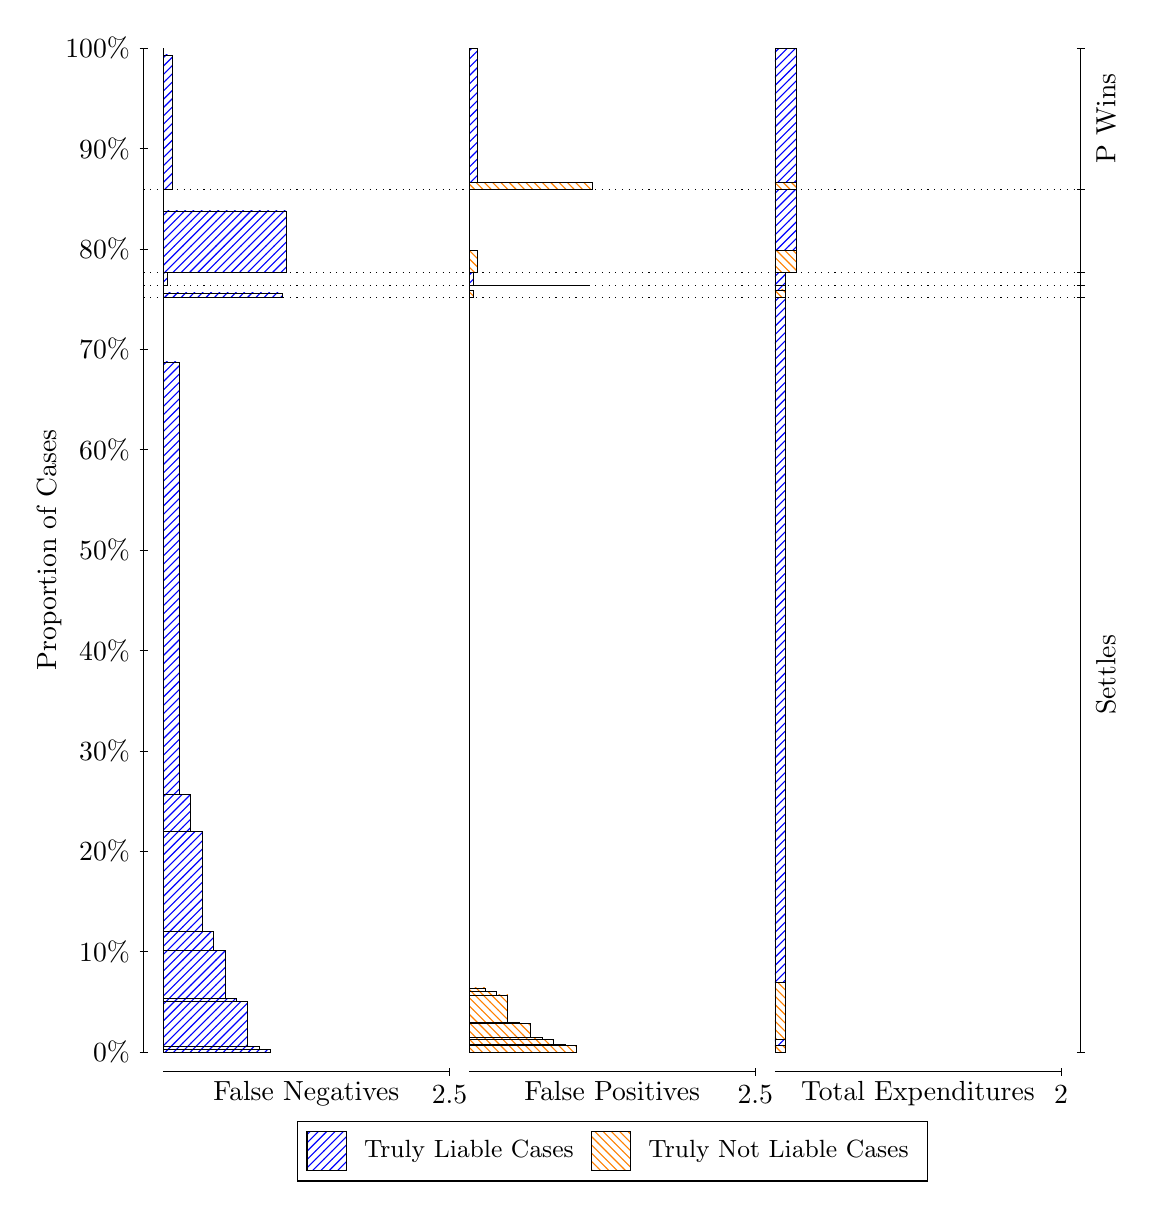
\begin{tikzpicture}
\draw[black, very thin] (1.5,1.75) -- (1.5,14.5);
\node[rotate=90, text=black, anchor=center] at (0.3, 8.125) {Proportion of Cases};
\draw[black, very thin] (1.45,1.75) -- (1.55,1.75);
\node[text=black, anchor=east] at (1.45, 1.75) {0\%};
\draw[black, very thin] (1.45,3.025) -- (1.55,3.025);
\node[text=black, anchor=east] at (1.45, 3.025) {10\%};
\draw[black, very thin] (1.45,4.3) -- (1.55,4.3);
\node[text=black, anchor=east] at (1.45, 4.3) {20\%};
\draw[black, very thin] (1.45,5.575) -- (1.55,5.575);
\node[text=black, anchor=east] at (1.45, 5.575) {30\%};
\draw[black, very thin] (1.45,6.85) -- (1.55,6.85);
\node[text=black, anchor=east] at (1.45, 6.85) {40\%};
\draw[black, very thin] (1.45,8.125) -- (1.55,8.125);
\node[text=black, anchor=east] at (1.45, 8.125) {50\%};
\draw[black, very thin] (1.45,9.4) -- (1.55,9.4);
\node[text=black, anchor=east] at (1.45, 9.4) {60\%};
\draw[black, very thin] (1.45,10.675) -- (1.55,10.675);
\node[text=black, anchor=east] at (1.45, 10.675) {70\%};
\draw[black, very thin] (1.45,11.95) -- (1.55,11.95);
\node[text=black, anchor=east] at (1.45, 11.95) {80\%};
\draw[black, very thin] (1.45,13.225) -- (1.55,13.225);
\node[text=black, anchor=east] at (1.45, 13.225) {90\%};
\draw[black, very thin] (1.45,14.5) -- (1.55,14.5);
\node[text=black, anchor=east] at (1.45, 14.5) {100\%};

\draw[black, very thin] (13.4,1.75) -- (13.4,14.5);
\draw[black, very thin] (13.35,1.75) -- (13.45,1.75);
\node[anchor=west] at (13.35, 1.75) {};
\draw[black, very thin] (13.35,11.329) -- (13.45,11.329);
\node[anchor=west] at (13.35, 11.329) {};
\draw[black, very thin] (13.35,11.488) -- (13.45,11.488);
\node[anchor=west] at (13.35, 11.488) {};
\draw[black, very thin] (13.35,11.654) -- (13.45,11.654);
\node[anchor=west] at (13.35, 11.654) {};
\draw[black, very thin] (13.35,12.707) -- (13.45,12.707);
\node[anchor=west] at (13.35, 12.707) {};
\draw[black, very thin] (13.35,14.5) -- (13.45,14.5);
\node[anchor=west] at (13.35, 14.5) {};

\draw[black, very thin, pattern color=blue, pattern=north east lines] (1.75,1.75) rectangle (3.1125,1.7802);
\draw[black, very thin, pattern color=blue, pattern=north east lines] (1.75,1.7802) rectangle (2.9672,1.8175);
\draw[black, very thin, pattern color=blue, pattern=north east lines] (1.75,1.8175) rectangle (2.8218,2.3919);
\draw[black, very thin, pattern color=blue, pattern=north east lines] (1.75,2.3919) rectangle (2.6765,2.4329);
\draw[black, very thin, pattern color=blue, pattern=north east lines] (1.75,2.4329) rectangle (2.5312,3.0383);
\draw[black, very thin, pattern color=blue, pattern=north east lines] (1.75,3.0383) rectangle (2.3858,3.2825);
\draw[black, very thin, pattern color=blue, pattern=north east lines] (1.75,3.2825) rectangle (2.2405,4.5538);
\draw[black, very thin, pattern color=blue, pattern=north east lines] (1.75,4.5538) rectangle (2.0952,5.0256);
\draw[black, very thin, pattern color=blue, pattern=north east lines] (1.75,5.0256) rectangle (1.9498,10.515);
\draw[black, very thin, pattern color=orange, pattern=north west lines] (1.75,10.515) rectangle (1.75,11.329);
\draw[black, very thin, pattern color=blue, pattern=north east lines] (1.75,11.329) rectangle (3.2578,11.389);
\draw[black, very thin, pattern color=orange, pattern=north west lines] (1.75,11.389) rectangle (1.75,11.488);
\draw[black, very thin, pattern color=blue, pattern=north east lines] (1.75,11.488) rectangle (1.8045,11.652);
\draw[black, very thin, pattern color=orange, pattern=north west lines] (1.75,11.652) rectangle (1.75,11.654);
\draw[black, very thin, pattern color=blue, pattern=north east lines] (1.75,11.654) rectangle (3.3123,12.433);
\draw[black, very thin, pattern color=orange, pattern=north west lines] (1.75,12.433) rectangle (1.75,12.707);
\draw[black, very thin, pattern color=blue, pattern=north east lines] (1.75,12.707) rectangle (1.859,14.414);
\draw[black, very thin, pattern color=orange, pattern=north west lines] (1.75,14.414) rectangle (1.75,14.5);
\draw[black, very thin, pattern color=orange, pattern=north west lines] (5.6333,1.75) rectangle (6.9958,1.8364);
\draw[black, very thin, pattern color=orange, pattern=north west lines] (5.6333,1.8364) rectangle (6.8505,1.8436);
\draw[black, very thin, pattern color=orange, pattern=north west lines] (5.6333,1.8436) rectangle (6.7052,1.9111);
\draw[black, very thin, pattern color=orange, pattern=north west lines] (5.6333,1.9111) rectangle (6.5598,1.9364);
\draw[black, very thin, pattern color=orange, pattern=north west lines] (5.6333,1.9364) rectangle (6.4145,2.1123);
\draw[black, very thin, pattern color=orange, pattern=north west lines] (5.6333,2.1123) rectangle (6.2692,2.1303);
\draw[black, very thin, pattern color=orange, pattern=north west lines] (5.6333,2.1303) rectangle (6.1238,2.4764);
\draw[black, very thin, pattern color=orange, pattern=north west lines] (5.6333,2.4764) rectangle (5.9785,2.5147);
\draw[black, very thin, pattern color=orange, pattern=north west lines] (5.6333,2.5147) rectangle (5.8332,2.5641);
\draw[black, very thin, pattern color=blue, pattern=north east lines] (5.6333,2.5641) rectangle (5.6333,11.329);
\draw[black, very thin, pattern color=orange, pattern=north west lines] (5.6333,11.329) rectangle (5.6878,11.428);
\draw[black, very thin, pattern color=blue, pattern=north east lines] (5.6333,11.428) rectangle (5.6333,11.488);
\draw[black, very thin, pattern color=orange, pattern=north west lines] (5.6333,11.488) rectangle (7.1412,11.49);
\draw[black, very thin, pattern color=blue, pattern=north east lines] (5.6333,11.49) rectangle (5.6878,11.654);
\draw[black, very thin, pattern color=orange, pattern=north west lines] (5.6333,11.654) rectangle (5.7423,11.928);
\draw[black, very thin, pattern color=blue, pattern=north east lines] (5.6333,11.928) rectangle (5.6333,12.707);
\draw[black, very thin, pattern color=orange, pattern=north west lines] (5.6333,12.707) rectangle (7.1957,12.793);
\draw[black, very thin, pattern color=blue, pattern=north east lines] (5.6333,12.793) rectangle (5.7423,14.5);
\draw[black, very thin, pattern color=orange, pattern=north west lines] (9.5167,1.75) rectangle (9.6529,1.8377);
\draw[black, very thin, pattern color=blue, pattern=north east lines] (9.5167,1.8377) rectangle (9.6529,1.9052);
\draw[black, very thin, pattern color=orange, pattern=north west lines] (9.5167,1.9052) rectangle (9.6529,2.6316);
\draw[black, very thin, pattern color=blue, pattern=north east lines] (9.5167,2.6316) rectangle (9.6529,11.329);
\draw[black, very thin, pattern color=orange, pattern=north west lines] (9.5167,11.329) rectangle (9.6529,11.428);
\draw[black, very thin, pattern color=blue, pattern=north east lines] (9.5167,11.428) rectangle (9.6529,11.488);
\draw[black, very thin, pattern color=orange, pattern=north west lines] (9.5167,11.488) rectangle (9.6529,11.49);
\draw[black, very thin, pattern color=blue, pattern=north east lines] (9.5167,11.49) rectangle (9.6529,11.654);
\draw[black, very thin, pattern color=orange, pattern=north west lines] (9.5167,11.654) rectangle (9.7892,11.928);
\draw[black, very thin, pattern color=blue, pattern=north east lines] (9.5167,11.928) rectangle (9.7892,12.707);
\draw[black, very thin, pattern color=orange, pattern=north west lines] (9.5167,12.707) rectangle (9.7892,12.793);
\draw[black, very thin, pattern color=blue, pattern=north east lines] (9.5167,12.793) rectangle (9.7892,14.5);
\draw[black, dotted] (1.5,11.329) -- (13.4,11.329);
\draw[black, dotted] (1.5,11.488) -- (13.4,11.488);
\draw[black, dotted] (1.5,11.654) -- (13.4,11.654);
\draw[black, dotted] (1.5,12.707) -- (13.4,12.707);
\draw[black, very thin] (1.75,1.5) -- (5.3833,1.5);
\node[text=black, anchor=north] at (3.5667, 1.5) {False Negatives};
\draw[black, very thin] (5.3833,1.45) -- (5.3833,1.55);
\node[text=black, anchor=north] at (5.3833, 1.45) {2.5};

\draw[black, very thin] (5.6333,1.5) -- (9.2667,1.5);
\node[text=black, anchor=north] at (7.45, 1.5) {False Positives};
\draw[black, very thin] (9.2667,1.45) -- (9.2667,1.55);
\node[text=black, anchor=north] at (9.2667, 1.45) {2.5};

\draw[black, very thin] (9.5167,1.5) -- (13.15,1.5);
\node[text=black, anchor=north] at (11.333, 1.5) {Total Expenditures};
\draw[black, very thin] (13.15,1.45) -- (13.15,1.55);
\node[text=black, anchor=north] at (13.15, 1.45) {2};

\node[text=black, centered, rotate=90] at (13.72, 6.5396) {Settles};



\node[text=black, centered, rotate=90] at (13.72, 13.603) {P Wins};

\draw (7.449999999999999,1.5) node[draw=none] (baseCoordinate) {};
\begin{scope}[align=center]
        \matrix[scale=0.5, draw=black, below=0.5cm of baseCoordinate, nodes={draw}, column sep=0.1cm]{
            \node[rectangle, draw, minimum width=0.5cm, minimum height=0.5cm, pattern color=blue, pattern=north east lines] {}; &
            \node[draw=none, font=\small, text=black] (B) {Truly Liable Cases}; &
            \node[rectangle, draw, minimum width=0.5cm, minimum height=0.5cm, pattern color=orange, pattern=north west lines] {}; &
            \node[draw=none, font=\small, text=black] (B) {Truly Not Liable Cases}; \\
            };
\end{scope}

\end{tikzpicture}
\end{document}